\subsection{Features}
A lot of features of \textit{Croc} are tied to the user interface, and for that reason it makes sense to present the \textit{Croc} UI.
%canvas features
In order to get an idea of how the \textit{Croc} UI looks like, see \figref{fig:croc-old-canvas}. 

\begin{figure}[h]
     \centering
     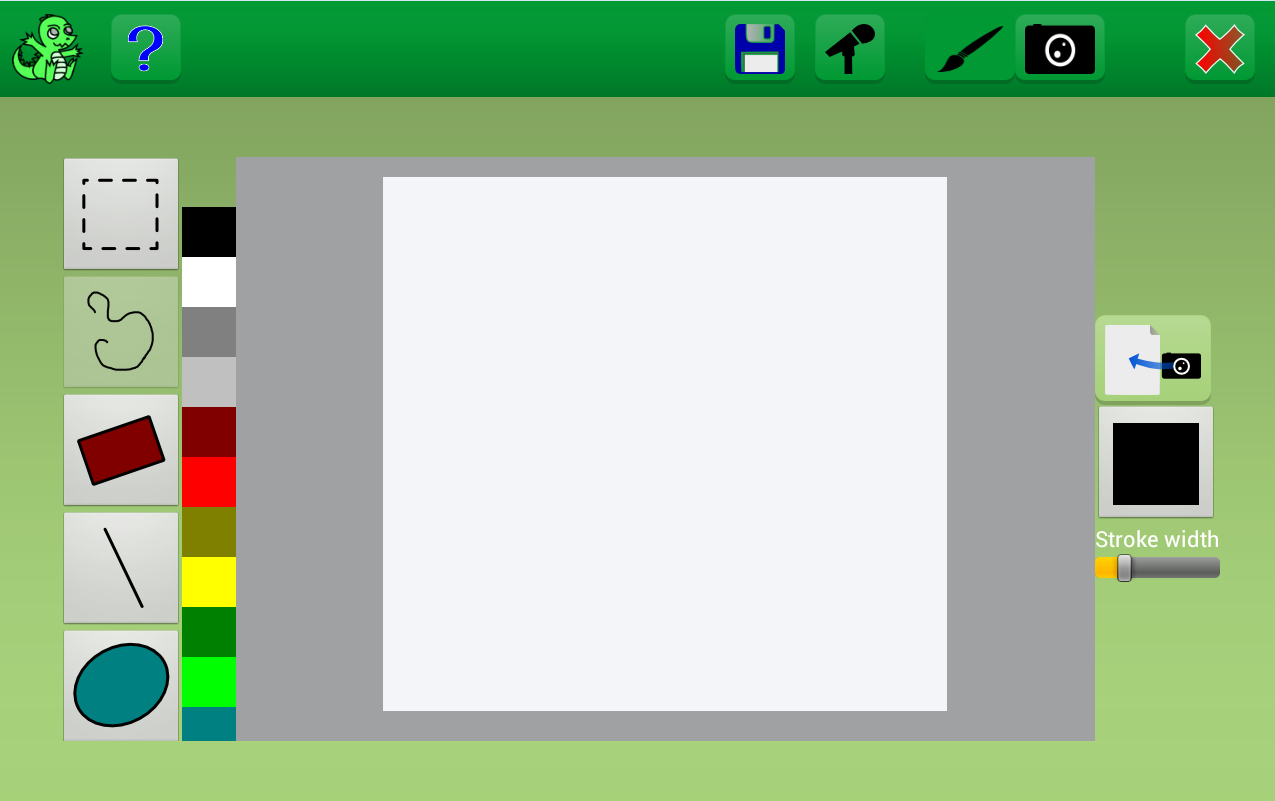
\includegraphics[scale=0.3]{CrocOldCanvas}
     \caption{Screenshot of canvas UI.}
     \label{fig:croc-old-canvas}
\end{figure}

The UI is divided into two parts, the upper serving as a menu-bar allowing access to the camera, audio recorder, help view, closing the application, or saving the pictogram.

The lower part changes depending on the mode chosen.
In the figure, the lower part shows the UI for the following features.

\begin{itemize}
     \item Selection
     \item Freehand, rectangle, line, and circle drawing
     \item Colour changing
     \item Load from Camera
     \item Colour preview
     \item Stroke width
\end{itemize}

Other features exists for the camera and audio recording, which include switching between black/white and colour pictures, take picture, start and end recording.
For screenshots of the camera and audio recorder, see \appref{app:crocUI}.